% No early warning. Build: tectonic paper.tex (figure: figs.py; every number: facts.json, written by build_facts.py)
\documentclass[10pt]{article}
\usepackage[letterpaper,margin=1.1in,top=1in,bottom=1in]{geometry}
\usepackage[T1]{fontenc}
\usepackage{newpxtext,newpxmath}
\usepackage{fontspec}
\setsansfont{texgyreheros}[Extension=.otf,UprightFont=*-regular,BoldFont=*-bold,ItalicFont=*-italic,BoldItalicFont=*-bolditalic,Scale=MatchUppercase]
\usepackage{microtype,graphicx,booktabs,xcolor,titlesec,enumitem}
\usepackage[font=small,labelfont=bf,skip=6pt]{caption}
\usepackage[numbers,sort&compress]{natbib}
\setlength{\bibsep}{0.5pt}
\definecolor{link}{HTML}{1D4ED8}
\usepackage[colorlinks,allcolors=link]{hyperref}
\titleformat{\section}{\sffamily\bfseries\large}{\thesection}{0.6em}{}
\titleformat{\subsection}{\sffamily\bfseries\normalsize}{\thesubsection}{0.6em}{}
\titlespacing*{\section}{0pt}{1.1em}{0.35em}
\titlespacing*{\subsection}{0pt}{0.8em}{0.25em}
\setlength{\parskip}{0.45em}\setlength{\parindent}{0pt}
\setlist{nosep,leftmargin=1.4em}
\newcommand{\ci}[2]{$[#1,\,#2]$}
\frenchspacing

\begin{document}

\begin{center}
{\sffamily\bfseries\LARGE No Early Warning\par}
\vspace{0.4em}
{\sffamily\large A critic that knew at token 1{,}000 which attempt will fail would be worth an RL run's gain.\\ In the first 2{,}000 tokens nothing we tried separates two attempts at one problem with an AUROC above 0.58;\\ the signal arrives when attempts end\par}
\vspace{1.0em}
{\large The Invariant Swarm}\\[0.25em]
{\small \href{https://monitor.invariant.team}{monitor.invariant.team} \quad$\cdot$\quad November 2026}
\end{center}

\vspace{0.2em}
\begin{center}\begin{minipage}{0.88\textwidth}
\small
\textbf{Abstract.} A base language model that is sampled four times on a math problem often gets it right in some
samples and wrong in others. If a critic could tell early which attempt will fail, the model could stop and start
again. On MATH-500, for the Olmo~3~7B base model with a short fixed opening, a perfect critic that looks once at
token 1{,}000 would raise the score from 410.5 to at most 459.2 of 500 at the same token cost; the model trained
with reinforcement learning (RL) scores 460.0. We looked for that critic. Bulut showed that early probes of
correctness predict how hard the problem is, not whether one attempt will succeed; we find the same on a base model and follow the question to
the end of the answer. Between two attempts at one problem, a linear probe on activations scores an AUROC of
0.50 at the prompt and at best 0.57 \ci{0.51}{0.63} at 1{,}000 tokens, and a restart policy driven by it gains
0.8 points \ci{-0.7}{2.4} over stopping at random. The signal that does appear is length: knowing which attempts have
ended gives 0.57 at token 4{,}000, and the final length gives 0.68. Abandoning any attempt still running at token
4{,}000 for one fresh attempt, with no critic, gains 1.2 points \ci{0.6}{1.7} for 22\,\% more tokens. Agreement among four finished answers scores 0.89.
\end{minipage}\end{center}

\begin{figure}[h]
\centering
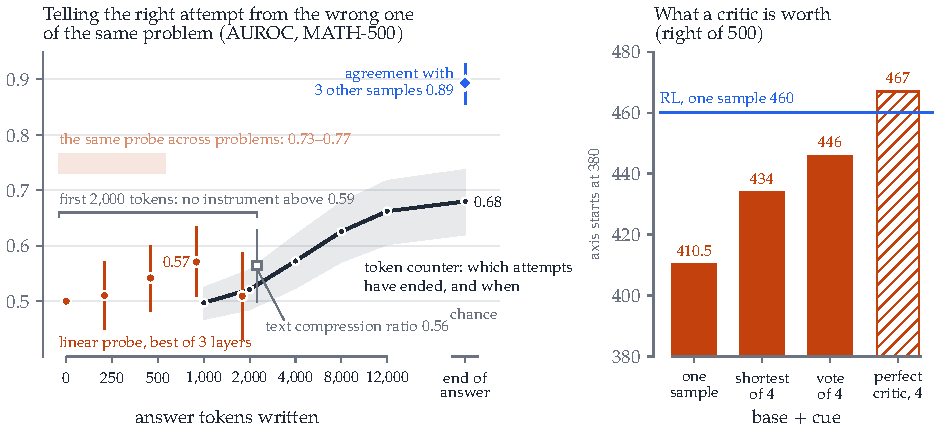
\includegraphics[width=\textwidth]{fig_warning.pdf}
\caption{\textbf{No early warning.} Olmo~3~7B base with a fixed opening, MATH-500, four samples per problem at
temperature 1.0. \textbf{Left:} how well each instrument orders a right and a wrong attempt at the same problem
(AUROC, the share of such pairs ordered correctly; 0.5 is chance; 478 pairs or fewer), against how much of the
answer is written. Probe points: the best of three layers at each position, against the agreement target.
Bands and bars: 95\,\% intervals.
\textbf{Right:} right answers of 500 for one sample, for three ways of choosing among four samples (the hatched
bar needs the answer key), and for the RL model.}
\label{fig:warning}
\end{figure}

\section{Introduction}

David \cite{david2025temporal} reports that a linear probe on a reasoning model's hidden state predicts whether
the answer will be right with an AUROC (area under the ROC curve) of 0.84, four tokens into the answer. Related
probes predict it from the prompt alone, with accuracy 60 to 76\,\% \cite{afzal2025knowing}, and at intermediate
answers, with AUROC above 0.7 \cite{zhang2025reasoning}. Such a probe suggests early stopping: abandon the
attempts that will fail. Bulut \cite{bulut2026problem} tested what these probes read. On 22 problems with 256
samples each from a distilled reasoning model, a pooled AUROC of 0.85 at token 4 fell to 0.50 \ci{0.47}{0.53}
within problems, and stayed at chance at all ten positions up to 512 tokens: the probe reads the difficulty of
the problem.

We ask the same question where the answer has a known value. Yue et al.\ \cite{yue2025does} showed that a base
model solves, in some of its samples, nearly all of what its RL-trained version solves. So a \emph{critic}, any
rule that scores an unfinished attempt, is worth about what RL is worth if it can tell attempts apart, and we
can state that value in problems and tokens. We then measure every instrument we have, within problems, from
the prompt to the end of the answer.

Our contribution is narrow. The within-problem comparison is Bulut's. New here are a base model at temperature 1.0, positions up
to the end of the answer, restart policies compared with random stopping and with a plain token counter, and
the value of the critic set against a released RL model.

\section{Setup}

\textbf{Models.} The base is Olmo~3~7B before any fine-tuning \cite{ettinger2025olmo}; the RL model is
Olmo~3.1~7B RL-Zero-Math, trained from that base. The base answers with a fixed three-token opening that ends in
``Okay'' prefilled (the \emph{cue}), a variant of the cue of Wang et al.\ \cite{wang2026base}; without it the
base rarely reasons step by step. The RL model gets the plain prompt.

\textbf{Samples.} MATH-500 \cite{hendrycks2021measuring,lightman2023lets}, four samples per problem at temperature
1.0 and top-$p$ 1.0, at most 16{,}384 generated tokens, the final boxed or marked answer checked against the reference with Math-Verify. Of the
base's 2{,}000 samples 1{,}642 are right; their median length is 1{,}950 tokens. On 150 problems the four
samples disagree in outcome; these give 478 pairs of one right and one wrong attempt at the same problem.

\textbf{Within-problem AUROC.} For an instrument that gives each sample a score, this is the share of those pairs
in which the right attempt has the better score. Any score that depends only on the problem gets exactly 0.5.
Intervals are 95\,\% from a bootstrap over problems. A planted score (correctness plus unit noise) gives 0.76;
lengths shuffled within problems give 0.49 \ci{0.43}{0.55}.

\textbf{Instruments.} (i) A logistic probe on the residual stream at layers 12, 20 and 28, at the last prompt token
and after 250, 500, 1{,}000 and 2{,}000 answer tokens, with five folds split by problem. It is trained on a
target that needs no answer key: whether the sample's final answer agrees with the largest group among the four
(the \emph{agreement target}), which equals correctness on 96.5\,\% of samples. (ii) Mean token entropy and
log-probability so far. (iii) The compression ratio of the text so far, a sign of repetition. (iv) The token
counter, $\min(\text{length}, t)$: at token $t$ it knows only which attempts have ended, and when. (v) At the
end: the final length, and agreement with the other three samples. Instruments (i) to (iii) at position $t$ use
only samples that reach $t$, so later positions have fewer pairs; the token counter uses all samples, and
between two attempts both still running it is 0.5 by construction.

\section{What the critic would be worth}

One sample of the base scores 410.5 of 500 and uses 4{,}008 tokens per problem. The RL model scores 460.0 with
4{,}687. Choosing among the base's four samples (Figure~\ref{fig:warning}, right): the shortest finished answer
gives 434, the majority answer 446, and a perfect critic 467, which is $+1.4$ points \ci{-0.1}{2.9} against
one RL sample. The vote is 2.8 points below RL \ci{-4.7}{-1.0} and costs four full answers, 16{,}034 tokens.

An early critic would remove that cost. We replay the stored samples: a critic reads the answer key once at
token 1{,}000 and restarts a failing attempt that is still running, up to four attempts. It reaches 459.2
\ci{447.9}{469.9} at 4{,}013 tokens per problem, $-0.2$ points \ci{-1.7}{1.4} against RL. This is an upper
bound, not a method: it assumes that at token 1{,}000 the outcome can already be known, which at temperature
1.0 need not be true. Nor does it capture all that RL adds: the same critic on the RL model's own samples reaches 481.8.

\section{The first 2{,}000 tokens}

\textbf{At the prompt.} Before any answer token, the probe separates right from wrong samples pooled over problems
with AUROC 0.73 to 0.77. Within a problem it scores exactly 0.5, as it must: the four attempts share one prompt.
The pooled number is no better than difficulty itself. Scoring each sample by the RL model's solve rate on its
problem gives 0.76, and by the base's other three samples 0.80.

\textbf{After the answer starts.} There are twelve probe cells (three layers, four positions). Against the
agreement target, one has an interval that excludes 0.5, uncorrected for the twelve comparisons: layer 12 at
1{,}000 tokens, 0.57 \ci{0.51}{0.63} on 340 pairs. Against correctness that cell scores 0.58 \ci{0.52}{0.65},
and layer 12 at 500 tokens, 0.56 \ci{0.51}{0.62}, also excludes 0.5; trained on shuffled labels the cell scores
0.50. At 2{,}000 tokens no layer exceeds 0.51 against the agreement target, or 0.55 \ci{0.48}{0.62} against
correctness. Entropy so far scores 0.57 \ci{0.51}{0.63} at 250 tokens against the agreement target (0.52
\ci{0.46}{0.58} against correctness) and 0.49 at 2{,}000. The compression ratio of the first 6{,}000 characters,
about 2{,}000 tokens, scores 0.56 \ci{0.50}{0.63}. So a weak signal may exist, near 0.55 to 0.58; with these
counts we can exclude only an AUROC above about 0.65.

\textbf{As a policy.} Stopping at token 1{,}000 the attempts that the probe scores below a threshold fitted on the
other folds, and restarting them, gives 414.1 of 500 at 4{,}345 tokens per problem. Stopping the same number of
attempts at random gives 410.1. The difference is 4.0 problems, 0.8 points \ci{-0.7}{2.4}, against the 49
problems (9.8 points) that a perfect critic adds at that position. We had predicted at least 420 at no more than
1.3 times the tokens, a gain over random stopping whose interval excludes zero, and a within-problem AUROC of at
least 0.60. All three predictions failed.

\section{The rest of the answer}

\textbf{Length.} By token 1{,}000, 28\,\% of attempts have ended, and by token 4{,}000, 69\,\%. Knowing which
have ended tells nothing at 1{,}000 and 2{,}000 tokens (0.50 and 0.52 \ci{0.48}{0.56}). At 4{,}000 tokens it
scores 0.57 \ci{0.52}{0.62}; at 8{,}000, 0.63 \ci{0.57}{0.68}; at 12{,}000, 0.66 \ci{0.60}{0.72}; and the final
length, 0.68 \ci{0.62}{0.74}. The attempt that runs long is the one more likely to fail. Between two attempts
both still running at token 1{,}000, the right one ends first in 73\,\% of the 373 pairs (AUROC 0.73
\ci{0.67}{0.79}), so most of this signal arises after token 1{,}000. We could not
test whether the probe's 0.57 is a forecast of that length: its scores are not stored per sample. On a harder
set of 328 problems the final length scores 0.65 \ci{0.58}{0.72}.

\textbf{Acting on length.} Forcing every attempt still running at 4{,}000 tokens to state its answer changes the score by $-3.6$
points \ci{-6.2}{-1.2} (one sample): of the 145 attempts cut, 70 would have ended right and 52 do so when forced.
At 8{,}000 tokens forcing changes nothing ($+0.2$ \ci{-1.0}{1.4}). Restarting helps a little. With no critic,
abandoning any attempt still running at token 4{,}000 and taking one fresh attempt gains 1.2 points
\ci{0.6}{1.7} for 22\,\% more tokens (4{,}886 per problem). Against one sample, the probe's policy gains 0.7
points for 8\,\% more tokens.

\textbf{Agreement.} Whether an attempt's answer agrees with the other three orders attempts with AUROC 0.89
\ci{0.85}{0.93}, and 0.83 on the harder set. It needs no answer key, and it is the vote of
Figure~\ref{fig:warning}. It needs every attempt finished, so it cannot stop one early.

\section{Related work}

Bulut \cite{bulut2026problem} is the closest work and has the same control; his within-problem test ends at 512
tokens and does not test a probe-driven stopping policy. David \cite{david2025temporal} notes that the probed
state may encode the easiness of the question. Later in the answer, attempt-level signals are known: Orgad et
al.\ \cite{orgad2024llms} select among 30 samples with a probe at the answer tokens, and Yuan et al.\
\cite{yuan2026hidden} find that wrong traces differ from right ones of the same problem at the end of the trace
(their pooled probe also works at the first step). Xi et al.\ \cite{xi2026calibration} find that a pre-answer
probe selects barely better than a majority vote (0.778 against 0.771), and Subhnil et al.\
\cite{subhnil2026effectiveness} that a probe on four traces per problem barely beats the trace text. Our
measurements cover both ranges on one set of samples: no clear attempt-level signal early, a growing one
carried by length, and a strong one once answers can be compared.

\section{Limitations}

\begin{itemize}
\item One base model, one benchmark and a harder set of the same kind; four samples per problem.
\item The probe is linear, reads one position in one of three layers, stops at 2{,}000 tokens, and was trained on
labels pooled over problems. It was never trained on a within-problem contrast or tested on a planted
attempt-level direction. Our result bounds this probe, not what the activations hold; the intervals allow an
AUROC up to about 0.65.
\item The probe's scores are not stored per sample, so its numbers are taken from the run's readout. Length,
agreement, compression ratio, all ceilings and the replays are recomputed from the stored samples.
\item The restart policies are replays on stored samples, not live runs.
\item The base has the cue and the RL model the plain prompt.
\item The forced-commit result is one sample.
\end{itemize}

\section{Conclusion}

For this base model an attempt-level critic at token 1{,}000 would be worth about the gain of an RL run, and no
early instrument we tried comes near it. Early, a probe reads the problem. What tells attempts apart later is
how long they run, and then whether they agree. A claim that a probe sees an attempt failing should be scored
within problems, and compared with a token counter.

{\small
\textbf{Reproducibility.} Code and the metrics of every run are in the team's repository, which is private and available on request, in the folder
\texttt{studies/rlneurons/}. In its folder \texttt{paper-no-warning/}, the script \texttt{build\_facts.py}
recomputes the numbers of this paper from the committed per-problem rows, or copies them from committed readouts
(probe, entropy, forced commit), and writes each with its source to
\texttt{facts.json}, and \texttt{figs.py} draws the figure.
}

{\small
\bibliographystyle{unsrtnat}
\bibliography{refs}
}

\end{document}
